
%
% STATE OF THE ART
%


\chapter{State of the art}

The 2-photon/confocal dataset that are produced in the Megason lab, are challenging.
They represent a lot of data, and have several artifacts that make image processing much harder.
Even though such confocal datasets are fairly recent, a lot of work has already been done for finding methods to robustly and efficiently process them.
This chapter presents the state of the art in the Megason lab,
namely, the data and techniques that already are available, as well as the techniques employed in other laboratories for objects detection in microscopy images.

%%%%%%%%%%%%%%%%%%%%%%%%%%%%%%%%%%%%%%%%%%%%%%%%%%%%%%%%%%%%%%%%%%%%%%%%%%%%%%%
%%%%%%%%%%%%%%%%%%%%%%%%%%%%%%%%%%%%%%%%%%%%%%%%%%%%%%%%%%%%%%%%%%%%%%%%%%%%%%%
%%%%%%%%%%%%%%%%%%%%%%%%%%%%%%%%%%%%%%%%%%%%%%%%%%%%%%%%%%%%%%%%%%%%%%%%%%%%%%%


\section{Challenges of data sets to be processed}
\label{setc:ChallengesData}
Biologists acquire tremendous amount of data (see table~\ref{tab:DataSizes})
corresponding in three dimensional videos of zebra fishes embryos
(see figure~\ref{fig:zebraconfoc}).

\subsection{Large amount of data}

We are working on fluorescent microscopy images acquired with a 2-photons confocal microscope. The acquisition process produces huge datasets that we must process efficiently.
Here is a small description of the images :
\begin{figure}[htb]
\begin{center}
\begin{tabular}{|c|c|c|}
\hline Dimension & Size & Resolution \\ 
\hline x (space) & 1024 & 0.24 um \\ 
\hline y (space) & 1024 & 0.24 um \\ 
\hline z (space) & 70 & 1 um \\ 
\hline t (time) & 700 & 2 min\\ 
\hline \multicolumn{3}{|c|}{ 2 intensity channels} \\ 
\hline
\end{tabular} 
\end{center}
\caption{Megason Lab typical fluorescent microscopy dataset}
\label{tab:DataSizes}
\end{figure}
The table~\ref{tab:DataSizes}, shows that the datasets are huge ( the intensity values are coded with {\verb+unsigned char+}, so that a full two channel dataset is approximatively  10.5 Gbit).

Those datasets include nuclei and membrane information in two different intensity channels, and in the future, will include more channels with other biological markers. 


\subsection{Complex data}
\begin{figure}[htb]
  \centering
  \subfloat[nuclei channel]{\label{fig:InterlaceNuclei}\includegraphics[width=0.7\textwidth]{pictures/InterlacingNuclei}}\\
  \subfloat[membrane channel]{\label{fig:InterlaceMembrane}\includegraphics[width=0.7\textwidth]{pictures/InterlacingMembrane}}                
  \caption{Interlacing artefact on 2 photon confocal images. Views are x-y cuts of a 3D volume}
  \label{fig:InterlacingArtefact}
\end{figure}
The imaging technique is point to point, and a mechanical displacement is involved for moving from on point to another (mirror displacement in the xy plan, and stage displacement on the z axis). This leads to several artefacts and drawbacks :


%%%%%%%%%%%%%%%%%%%%%%%%%%%%%%%%%%%%%%%%%%%%%%%%%%%%%%%%%%%%%%%%%%%%%%%%%%%%%%%%

\subsubsection{Interlacing artefact}
This artefact is due to the microscope's raster scanning: it scans a line, following the x axis, and then increment on the y axis and scans another line.
The uncertainty on the x axis leads to interlacing of successive lines as illustrated figure~\ref{fig:InterlacingArtefact}.
This interlacing is also due to displacement uncertainties while scanning a line : as displacement varies, pixel width varies !
Thus this interlacing artefact is not isotropic: a line may seem to be translated of a positive factor on the right of the image, and of a negative factor on the left !


%%%%%%%%%%%%%%%%%%%%%%%%%%%%%%%%%%%%%%%%%%%%%%%%%%%%%%%%%%%%%%%%%%%%%%%%%%%%%%%%

\subsubsection{Anisotropy of images}
\begin{figure}[htb]
  \centering
  \captionsetup[subfloat]{labelformat=empty}
  \subfloat[][]{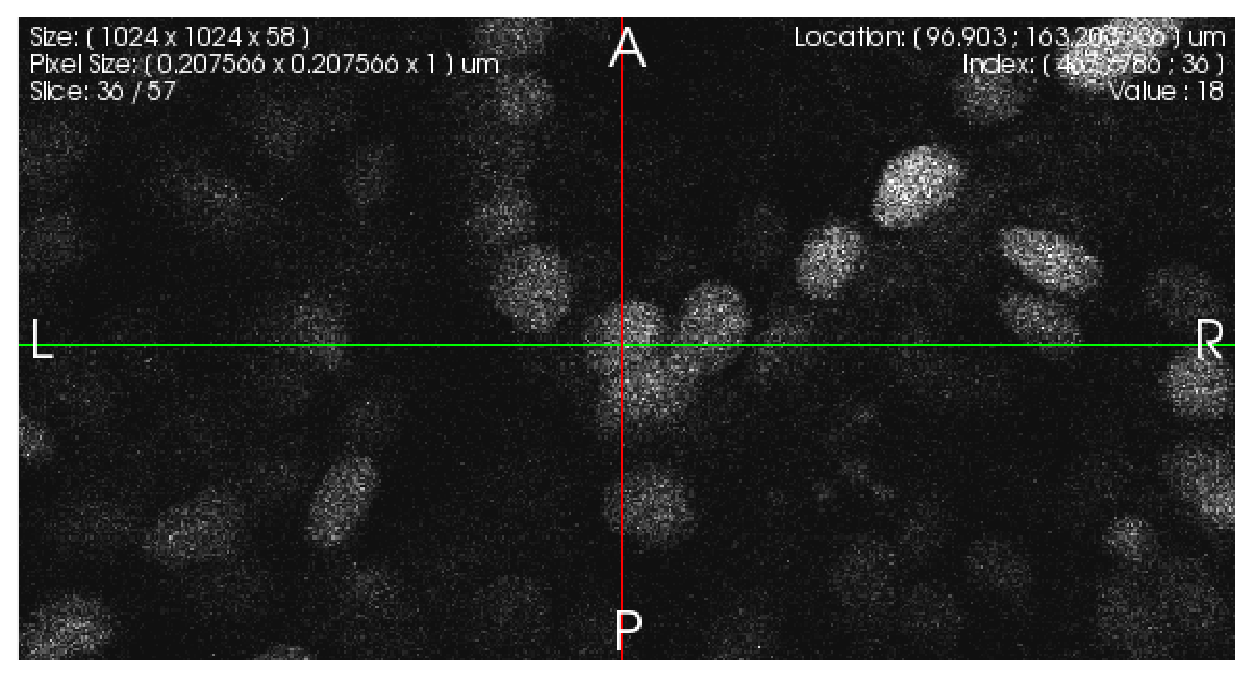
\includegraphics[width=0.7\textwidth]{pictures/anisotropieNucleiXY}\label{fig:anisotropieNucleiXY}}\\
  \subfloat[][]{{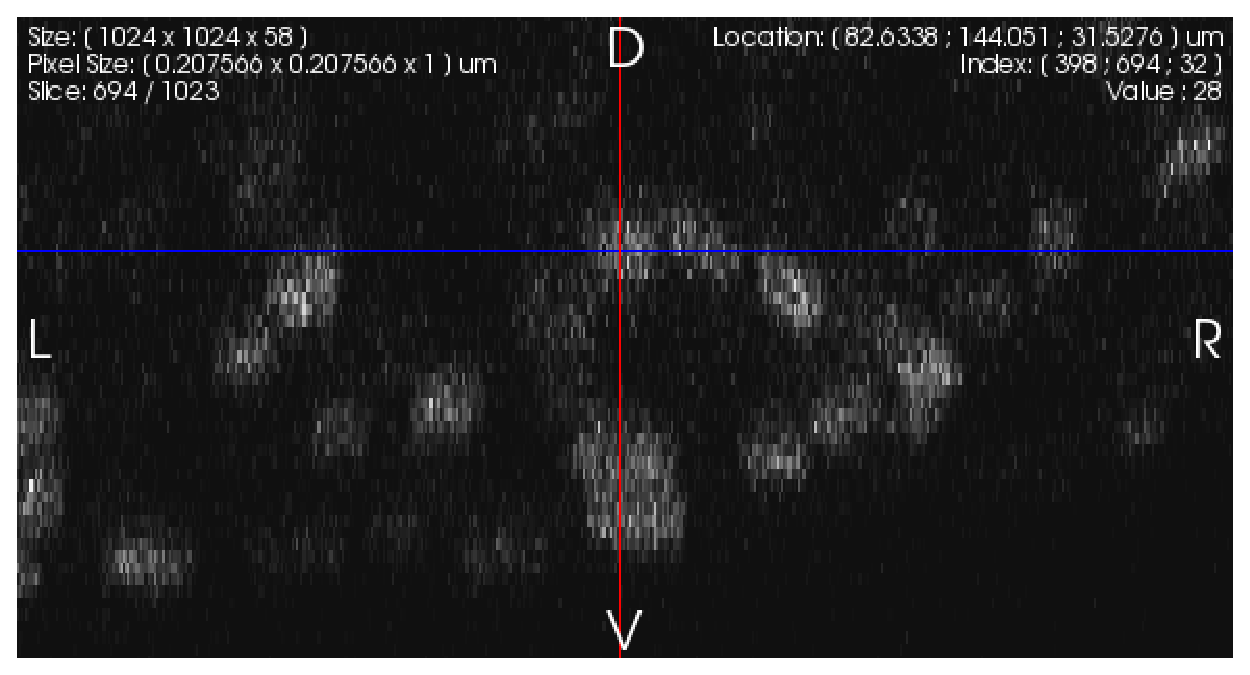
\includegraphics[width=0.7\textwidth]{pictures/anisotropieNucleiXZ}\label{fig:anisotropieNucleiXZ}}}
\caption{%
Illustration of the anisotropy of the datasets in the nuclei channel (view along xy~\subref{fig:anisotropieNucleiXY}, along xz~\subref{fig:anisotropieNucleiXZ}).}
\label{fig:anisotropy}
\end{figure}
\begin{figure}[htb]
  \centering
  \captionsetup[subfloat]{labelformat=empty}
  \subfloat[][]{{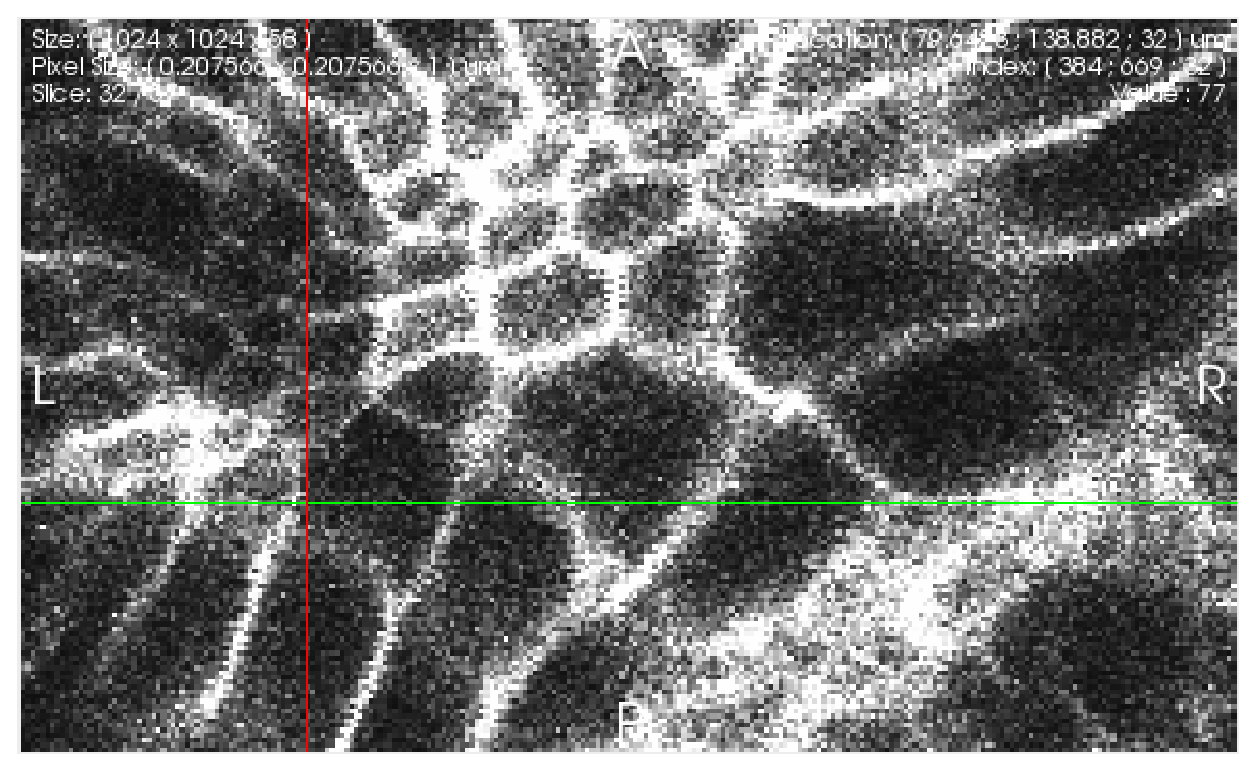
\includegraphics[width=0.7\textwidth]{pictures/anisotropieMembraneXY}\label{fig:anisotropieMembraneXY}}}\\
  \subfloat[][]{{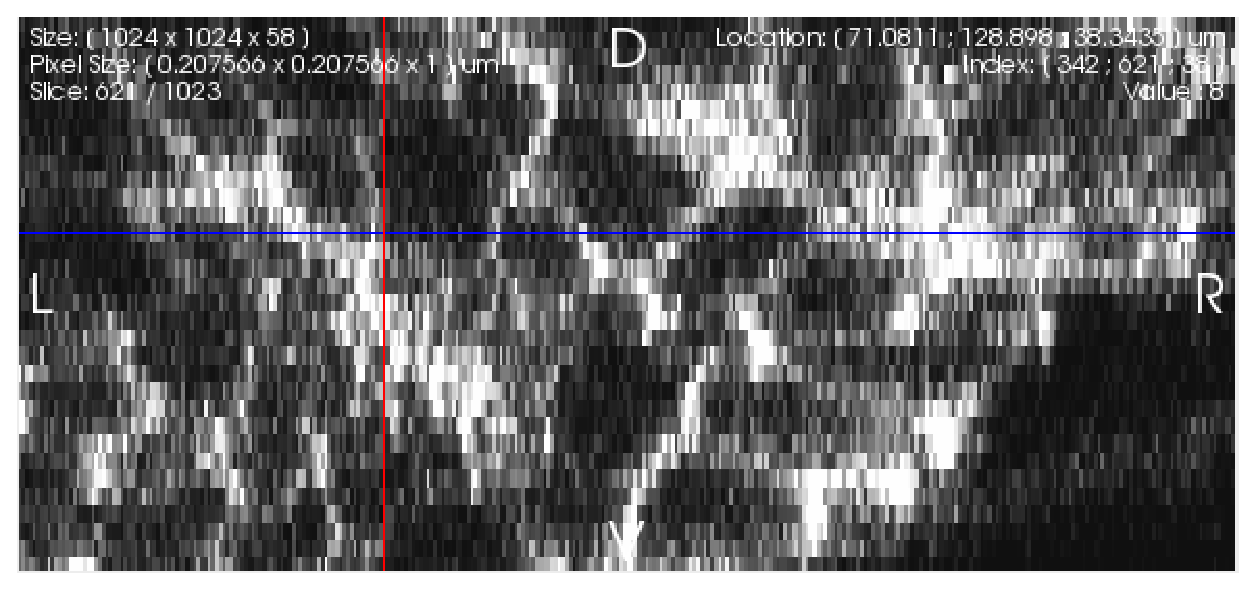
\includegraphics[width=0.7\textwidth]{pictures/anisotropieMembraneXZ}\label{fig:anisotropieMembraneXZ}}}
\caption{%
Illustration of the anisotropy of the datasets in the membrane channel (view along xy~\subref{fig:anisotropieMembraneXY}, along xz~\subref{fig:anisotropieMembraneXZ})}
\label{fig:anisotropy}
\end{figure}
The datasets acquired in the Megason lab are anisotropic. As in the medical imaging domain, specialists are used to analyse images "slice by slice"
instead of considering them as a volume. They are worried about having a very detailed image in the x-y plan, and don't really worry about the other dimension.
This way of seeing things is wrong for images processing. A completely anisotropic image is very hard to process.
Non existing structures appear in the third dimension as illustrated figure~\ref{fig:anisotropy}.
If a human brain with its understanding of the data may be able to interpret these structures, they lead most common algorithms to failure.
We can notice that nuclei seem to be stuck together and membrane's closure is almost always missing. This gives challenging a priori introduction problems.

Another challenging problem comes from inhomogeneous intensity as described in~\cite{umesh2001efficient}, along the z axis (see figure~\ref{fig:membraneHolesXZ}).



%%%%%%%%%%%%%%%%%%%%%%%%%%%%%%%%%%%%%%%%%%%%%%%%%%%%%%%%%%%%%%%%%%%%%%%%%%%%%%%%

\subsubsection{Noise}
There is much noise present in the datasets (see figure~\ref{fig:noiseNuc}). Both membrane channel and nuclei channel are populated with non Gaussian noise.
The noise comes both from the microscope and electronics acquisition equipments, and from the biological sample that can be fluorescent in random locations.
The acquisition noise along z axis is decorrelated.

The problem also comes from the fact that depending on the phosphor used, the noise's statistics will differ.
\begin{figure}[htb]
\centering
  \subfloat[][]{{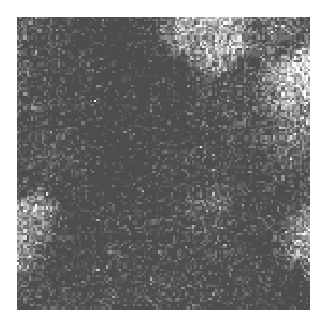
\includegraphics[width=0.3\textwidth]{pictures/noiseXY}\label{fig:noiseXY}}} \hspace{5pt}
  \subfloat[][]{{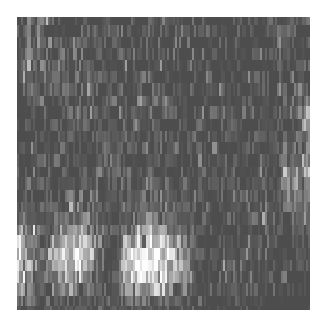
\includegraphics[width=0.3\textwidth]{pictures/noiseXZ}\label{fig:noiseXZ}}}
  \caption{%
    Illustration of the noise in the nuclei channel of confocal images.
    \subref{fig:noiseXY}: in a xy slice;
    \subref{fig:noiseXZ}: in a xz slice. 
    Notice, that \subref{fig:noiseXY} contains some nuclei as references, in the top right corner, and \subref{fig:noiseXZ} in the bottom left.}
\label{fig:noiseNuc}
\end{figure}



%%%%%%%%%%%%%%%%%%%%%%%%%%%%%%%%%%%%%%%%%%%%%%%%%%%%%%%%%%%%%%%%%%%%%%%%%%%%%%%%

\subsubsection{Low resolution of images}

The imaging process, combined with a too low resolution, leads to merged or missing structures.
The nuclei channel displays very often clusters of merged nuclei (see figure~\ref{fig:anisotropy})
when the membrane channel has information holes (see figure~\ref{fig:holesMembrane}).

\begin{figure}[htb]
  \centering
  \captionsetup[subfloat]{labelformat=empty}
  \subfloat[][]{{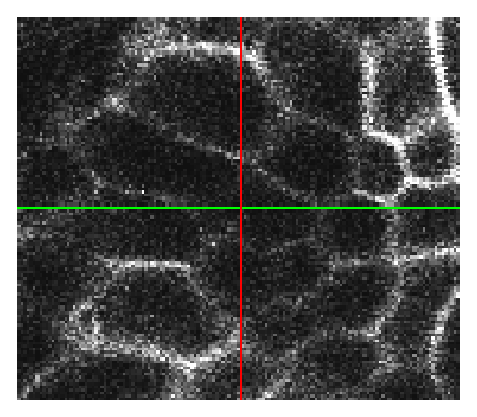
\includegraphics[width=0.45\textwidth]{pictures/membraneHolesXY}\label{fig:membraneHolesXY}}}\hspace{5pt}
  \subfloat[][]{{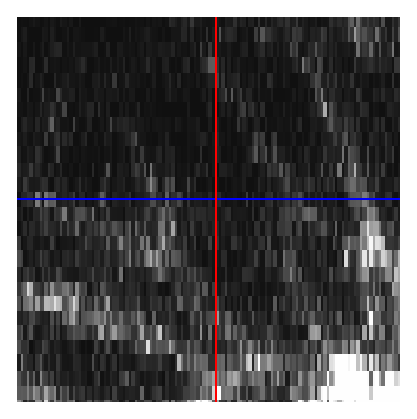
\includegraphics[width=0.45\textwidth]{pictures/membraneHolesXZ}\label{fig:membraneHolesXZ}}}
%\subfloat[][]{{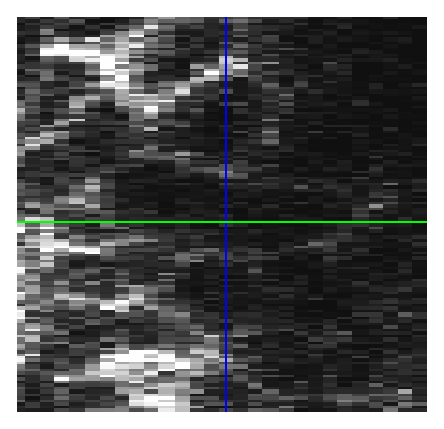
\includegraphics[width=0.7\textwidth]{pictures/membraneHolesYZ}\label{fig:membraneHolesYZ}}}
\caption{%
Illustration of missing information in the membrane channel. Holes and intensity inhomogeneities in a xy plan~\subref{fig:membraneHolesXY}, a xz plan~\subref{fig:membraneHolesXZ}.}
\label{fig:holesMembrane}
\end{figure}


%%%%%%%%%%%%%%%%%%%%%%%%%%%%%%%%%%%%%%%%%%%%%%%%%%%%%%%%%%%%%%%%%%%%%%%%%%%%%%%%

\subsubsection{Point spread function}
\begin{figure}[htb]
\begin{center}
\leavevmode
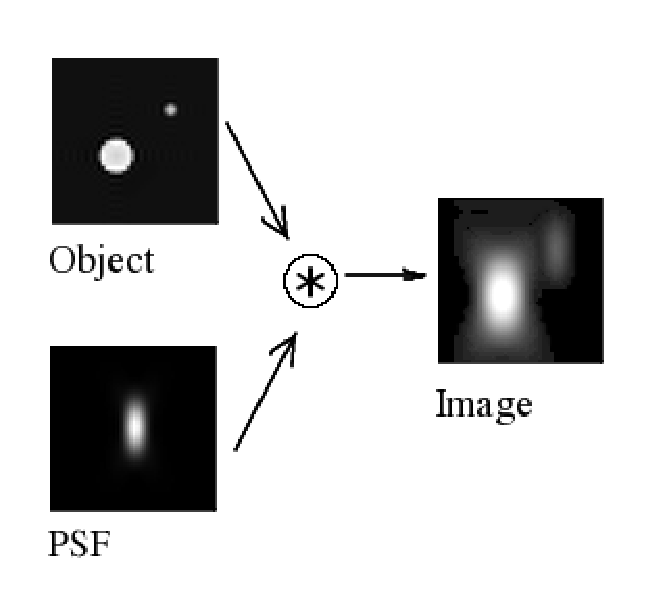
\includegraphics[width=0.3\textwidth]{pictures/pointSpreadFunction}
\end{center}
\caption{Illustration of the Point Spread Function (PSF) principle : the object is convoluted with the PSF. (source: \href{http://en.wikipedia.org/wiki/File:Convolution_Illustrated_eng.png}{Wikipedia})}
\label{fig:pointSpreadPrinciple}
\end{figure}
The impulse response of the microscope is a noisy point spread function (see figure~\ref{fig:pointSpreadPrinciple}).
That adds a deconvolution problem that can be treated together with the denoising problem.
For simplicity reasons, researchers image with a very low resolution along the z axis, as the impulse function is spread out a lot along this axis.
It is possible to correct such noise by knowing the impulse response of the microscope.
Knowing exactly this PSF, would give us the chance to have a better z resolution, by oversampling in z, and deconvolving.
For that purpose, we could image a sub-pixelic fluorescent object, and evaluate the impulse response of the whole system.



%%%%%%%%%%%%%%%%%%%%%%%%%%%%%%%%%%%%%%%%%%%%%%%%%%%%%%%%%%%%%%%%%%%%%%%%%%%%%%%%s

\subsubsection{Complex structures}

The images we get are complex assembly of cells.
Some area being full of membrane, and others full with inter cellular liquid.
This is not a simple microscope slide with some well known cells, but a whole developing organism.




\clearpage
%%%%%%%%%%%%%%%%%%%%%%%%%%%%%%%%%%%%%%%%%%%%%%%%%%%%%%%%%%%%%%%%%%%%%%%%%%%%%%%
%%%%%%%%%%%%%%%%%%%%%%%%%%%%%%%%%%%%%%%%%%%%%%%%%%%%%%%%%%%%%%%%%%%%%%%%%%%%%%%
%%%%%%%%%%%%%%%%%%%%%%%%%%%%%%%%%%%%%%%%%%%%%%%%%%%%%%%%%%%%%%%%%%%%%%%%%%%%%%%

\section{The Megason lab imaging pipeline}

Dr Kishore Mosaliganti has been working for two years in the Megason lab, in order to develop new segmentation methods for fluorescent images.
He has been working on experiencing and developing diverse algorithms for nuclei and membrane detection and segmentation.
As presented is the previous section, the datasets in the Megason Lab are extremely challenging:
they are huge and present important drawbacks (resolution, noise) as they are provided for visual processing and not computer assisted processing.

Kishore studied several algorithms for nuclei and membrane segmentation.
For nuclei segmentation, an approach based on detection of nuclei, and region growing with the level set theory was used last year.
This year, a new approach based on nuclei detection and watershed algorithms is being used.
The algorithm used are standard and contour based for the detection of nuclei.
This leads to many errors in detection, due to the poor image quality. Right now, these errors are compensated after the segmentation step.

For membrane segmentation, Kishore is proposing a very good denoising technique based on anisotropic diffusion~\cite{kishoreMembrane}, and tensor voting (not published yet).
The reconstruction of the membrane structure is effective, even in low quality images. A segmentation step has to be implemented on top of it.


\section{Existing methods for nuclei detection}

Cell nuclei shapes varies from spherical to curved ellipsoidal. As introduced above, the microscopy images are challenging, they are very noisy and anisotropic.
The main encountered difficulty is clustered nuclei that result from the point spread function of the microscope and the low resolution in the third dimension.

The algorithms used in the Megason lab for nuclei and membrane segmentation are based on an initialisation inside the nuclei.
Right now, a composite algorithm is used for detecting these nuclei based on a combination of contour based algorithms (see~\ref{sect:megasonExisting}).
This method gives good enough results for starting a watershed algorithm. Segmented regions that obviously don't correspond to a cell nucleus are eliminated. The final result of the segmentation process is evaluated.

There are several papers dealing with cell nuclei or cell detection 
\cite{loukas2003image,umesh2001efficient,al2009improved},
but only one is based on 3D 2-photon/confocal images~\cite{li20073},
similar to the ones acquired in the Megason lab.

\subsection*{Confocal nuclei detection}
G. Li {\etal}~\cite{li20073}, describe a segmentation method for nuclei in 3D confocal datasets. The method they use is based on gradient vector flow tracking.
The image processing pipeline is presented figure~\ref{fig:gradientflowFlowchart}.
\begin{description}
  \item[Data] are 3D confocal datasets from zebrafish embryos. They are fluorescent nuclei.
  \item[Method] is described figure~\ref{fig:gradientflowFlowchart}. 
  A re-sampling and spline based interpolation is performed on the original data to get isotropic datasets.
  The gradient vector diffusion field (see figure~\ref{fig:gradientflowFlowfield}) is then computed on a Gaussian blurred version of the isotropic data.
  Following \cite{bajcsy1989multiresolution}, an elastic constraint is added to the diffusion equation to get a smooth vector field.
  The tracking consists in selecting some points and moving them according to the vector field. The resulting trajectories end in "sinks" that correspond to center of nuclei.
  A refinement step groups the close "sinks".
  The segmentation is the done by cropping the image around each nuclei and applying a local adaptive threshold to find one nuclei per subregion.
  A final step consists in eliminating the false positives (nuclei which are too small).
  \item[Evaluation] is performed on 10 confocal datasets. The mean amount of nuclei in the datasets is 310. The number of over segmented and under segmented nuclei is presented. The automatic segmentation result is compared with the segmentation of two experts.
  \item[Results] the algorithm provides good results in the paper: 
  4.93\% of over-segmented nuclei,
  and 5.03\% of under-segmented nuclei.
  \item[Comments]:
  The article misses the part describing the region cropping for getting the regions where the adaptive
   threshold should be computed.
   Looking at the illustration, it seems like these regions are either determined
   according to attraction basins of each sink, or with a constrained Voronoi diagram.
\end{description}
\begin{figure}[h]
\begin{center}
\leavevmode
\includegraphics[height=0.87\textheight]{pictures/gradientflowFlowchart}
\end{center}
\caption{Flowchart of the algorithm proposed in~\cite{li20073}}
\label{fig:gradientflowFlowchart}
\end{figure}

\begin{figure}[h]
  \centering
  \captionsetup[subfloat]{labelformat=empty}
  \subfloat[][]{{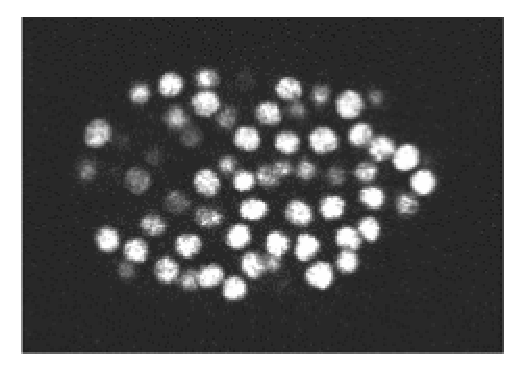
\includegraphics[width=0.33\textwidth]{pictures/gradientflowSegmenta}\label{fig:gradientflowSegmenta}}}
  \subfloat[][]{{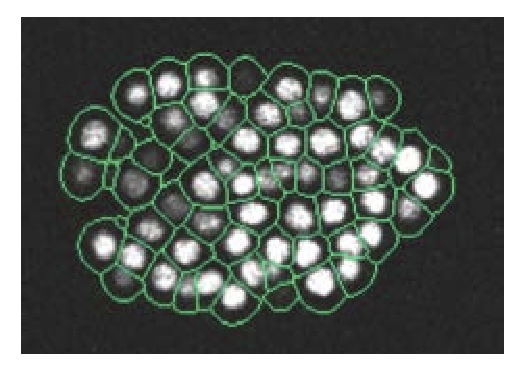
\includegraphics[width=0.33\textwidth]{pictures/gradientflowSegmentb}\label{fig:gradientflowSegmentb}}}\\
  \subfloat[][]{{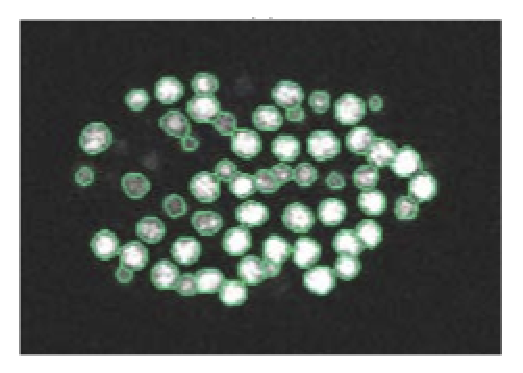
\includegraphics[width=0.33\textwidth]{pictures/gradientflowSegmentc}\label{fig:gradientflowSegmentc}}}
  \subfloat[][]{{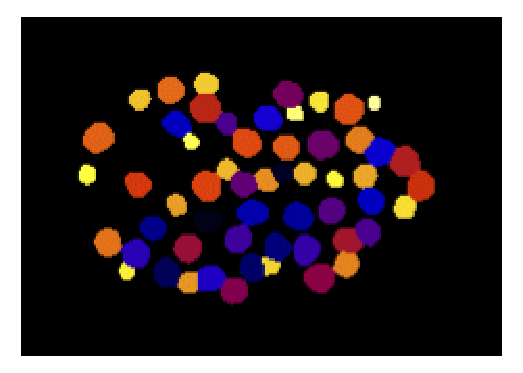
\includegraphics[width=0.33\textwidth]{pictures/gradientflowSegmentd}\label{fig:gradientflowSegmentd}}}
\caption{%
Illustration of 3D cell nuclei segmentation on a 2D slice, from~\cite{li20073}.
\subref{fig:gradientflowSegmenta}: A slice from 3D cell nuclei image;
\subref{fig:gradientflowSegmentb}: Boundaries of small regions overlaid on the slice;
\subref{fig:gradientflowSegmentc}: Edges of cell nuclei overlaid on the slice after the step of adaptive thresholding;
\subref{fig:gradientflowSegmentd}: Randomly color-coded extracted cells.}
\end{figure}

\begin{figure}[h]
  \centering
  \captionsetup[subfloat]{labelformat=empty}
  \subfloat[][]{{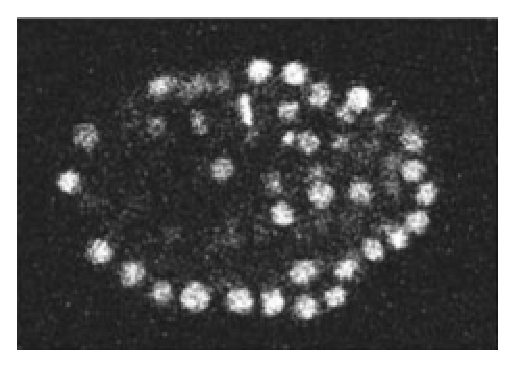
\includegraphics[width=0.5\textwidth]{pictures/gradientflowFlowfielda}\label{fig:gradientflowFlowfielda}}}\\
  \subfloat[][]{{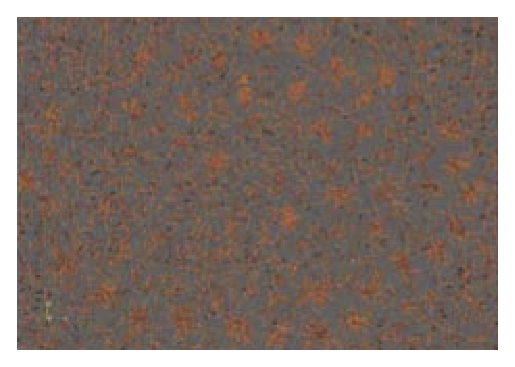
\includegraphics[width=0.33\textwidth]{pictures/gradientflowFlowfieldb}\label{fig:gradientflowFlowfieldb}}} \hspace{5pt}
  \subfloat[][]{{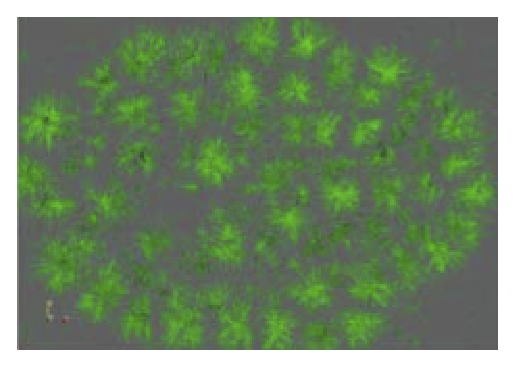
\includegraphics[width=0.33\textwidth]{pictures/gradientflowFlowfieldc}\label{fig:gradientflowFlowfieldc}}}\\
  \subfloat[][]{{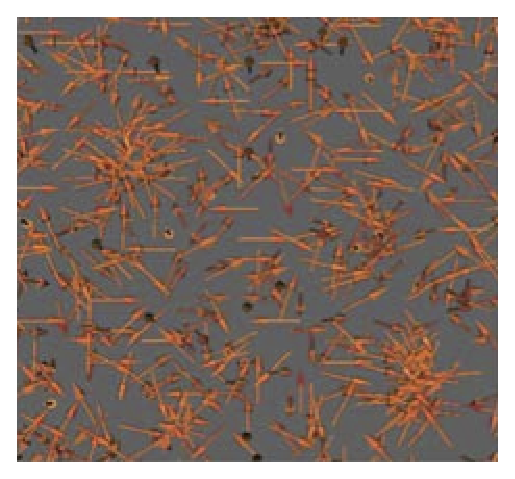
\includegraphics[width=0.33\textwidth]{pictures/gradientflowFlowfieldd}\label{fig:gradientflowFlowfieldd}}} \hspace{5pt}
  \subfloat[][]{{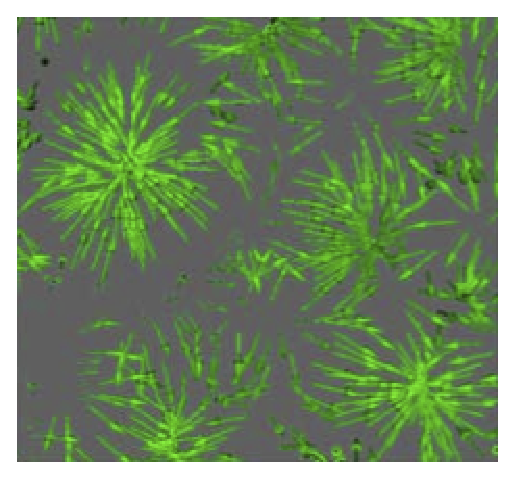
\includegraphics[width=0.33\textwidth]{pictures/gradientflowFlowfielde}\label{fig:gradientflowFlowfielde}}}
\caption{%
The 3D view of gradient vector field and diffused gradient vector field with elastic deformation transformation of a slice cropped from a 3D cell nuclei image, from~\cite{li20073}.
\subref{fig:gradientflowFlowfielda}: A slice of the 3D image;
\subref{fig:gradientflowFlowfieldb}: The original gradient vector field;
\subref{fig:gradientflowFlowfieldc}: The diffused gradient flow field with elastic deformation transformation;
\subref{fig:gradientflowFlowfieldd}: Zoomed view of \subref{fig:gradientflowFlowfieldb};
\subref{fig:gradientflowFlowfielde}: Zoomed view of \subref{fig:gradientflowFlowfieldc}.}
\end{figure}
\clearpage

\subsection*{3D histological pathological cell detection}
 P.S. Umesh Adiga {\etal}~\cite{umesh2001efficient}, present a method for segmenting cells in histological images 
  (which are somehow close to nuclei in fluorescent images).
  \begin{description}
  \item[Data] are 3D confocal histo-pathological images of cells in thick tissues.
  \item[Method] is described figure~\ref{fig:watershedFlowchart}.
  A first step consists in thresholding the image to keep only the nuclei. The threshold level is given by an empirical law based on the histogram of the images.
  Then, a succession of mathematical morphology operations consisting in opening and closing with a structuring element of same size, are used to improve the data. 
  This filters the texture of the cells, and removes holes.
  An intensity correction is then applied along the z axis. The figure~\ref{fig:watershedPrefilt} illustrates the results of this pre-processing.
  After a binarization of the preprocessed image, a distance map is computed and thresholded to find the cell markers, to initiate the watershed algorithm.
  Once the watershed algorithm has converged, a region merging process groups over-segmented cells. The region merge used in this paper is described by figure~\ref{watershedMerge}.
  \item[Evaluation] is performed on 15 3D datasets. The mean amount of nuclei in the datasets is 22. The information provided by the evaluation is the number of detected cells compared to the number of real cells present. No information is given on the type of error. The algorithm is compared to \cite{malpica1997applying}, and shows better performance according to the evaluation criterion.
  \item[Results] the algorithm provides very good results in the paper with 2\% of error instead of 9\% for \cite{malpica1997applying}.
  \item[Comments]: this article is well presented with a description of all the steps of the processing pipeline.
  The evaluation is done on small datasets (256*256*24) with few cells. A good information would have been amount of under segmented cells. 
\end{description}
\begin{figure}[h]
\begin{center}
\leavevmode
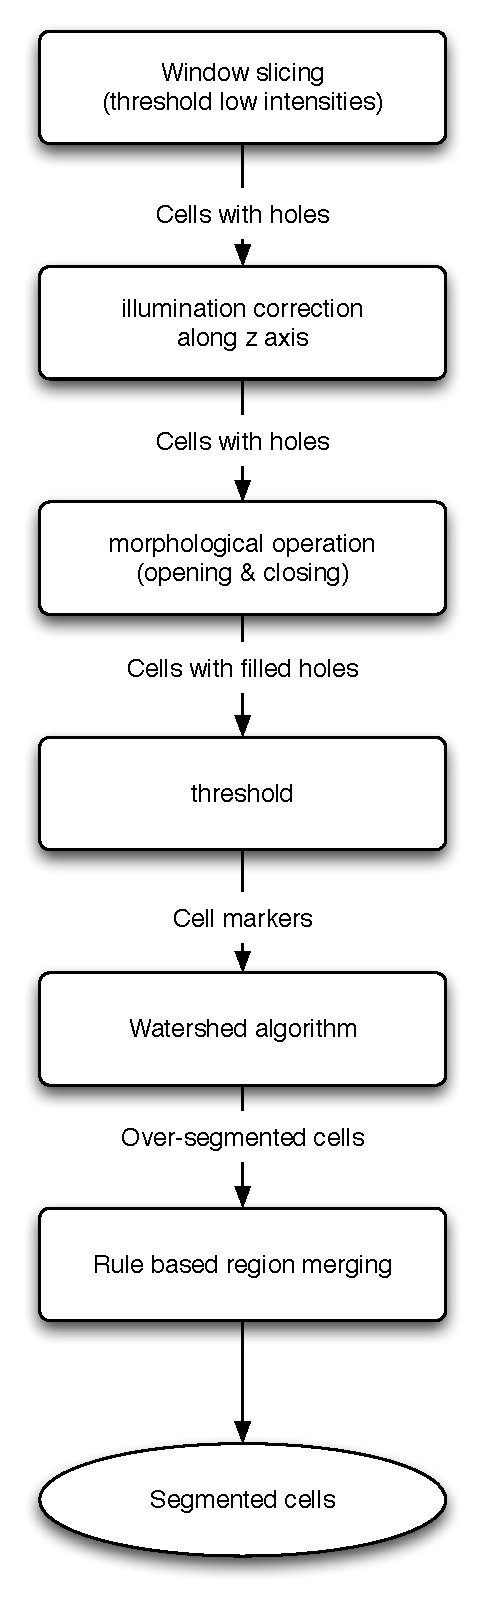
\includegraphics[height=0.87\textheight]{pictures/watershedFlowchart}
\end{center}
\caption{Flowchart of the algorithm proposed in~\cite{umesh2001efficient}}
\label{fig:watershedFlowchart}
\end{figure}

\begin{figure}[h]
  \centering
  \captionsetup[subfloat]{labelformat=empty}
%
  \subfloat[Diagrammatic representation of detecting the small fragments of the object and finding its parent.]%
{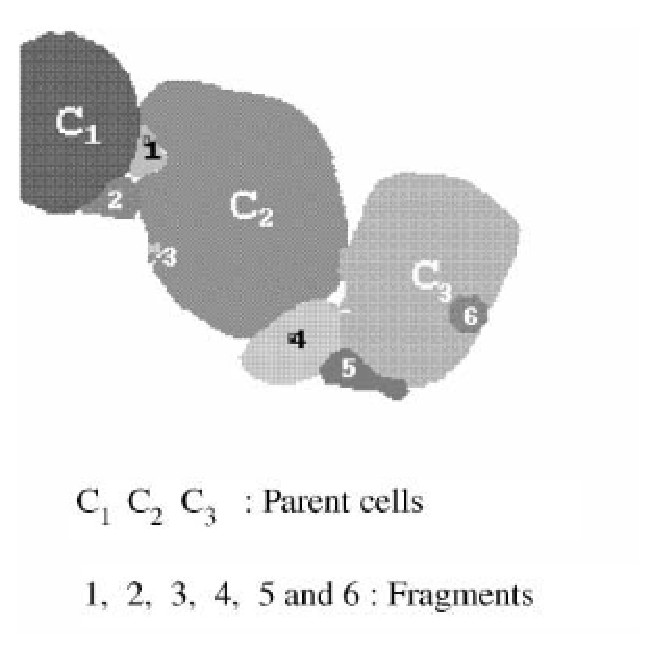
\includegraphics[width=0.47\textwidth]{pictures/watershedMergea}\label{fig:watershedMergea}}%
%
\subfloat[After merging the fragments.]%
{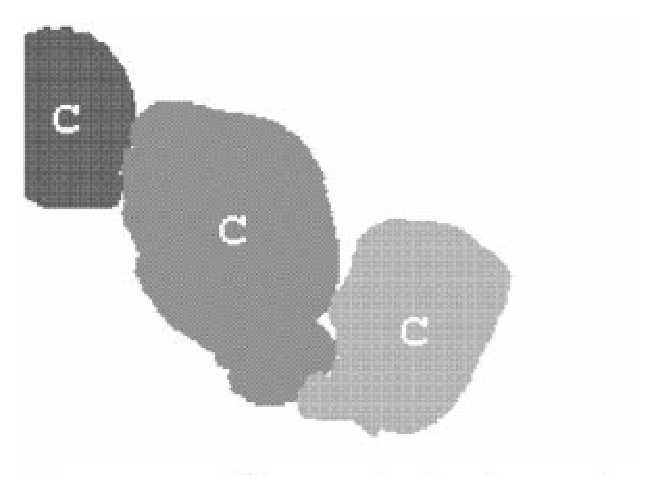
\includegraphics[width=0.47\textwidth]{pictures/watershedMergeb}\label{fig:watershedMergeb}}%
%
\caption{Illustrations from \cite{umesh2001efficient}: Merging of fragments :\\
Fragment 1 and 2 shares the boundary with \( C_1 \) and \( C_2 \) but fragments 1 shares maximum boundary with \( C_2 \) while fragment 2 shares maximum boundary with  {\( C_1 \)}. So fragment 1 is merged to  {\( C_2 \)}, 2 is merged to {\( C_1 \)}, 3 to {\( C_2 \)}, 4 to {\( C_2 \)}, 5 and 6 to {\( C_3 \)}.}
  \label{fig:watershedIllustration}
\end{figure}
\begin{figure}[h]
  \centering
  \captionsetup[subfloat]{labelformat=empty}
\subfloat[][]{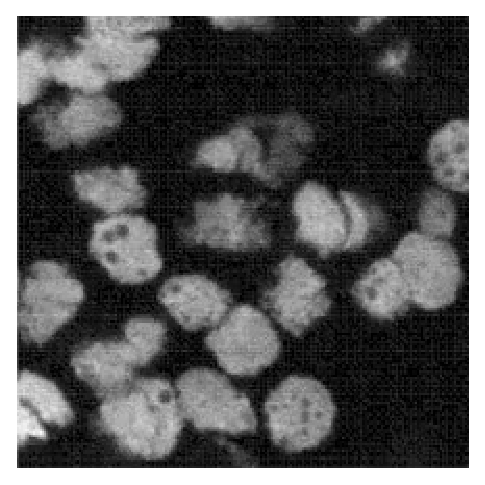
\includegraphics[width=0.33\textwidth]{pictures/watershedPrefilta}\label{fig:watershedPrefilta}}\hspace{5pt}
\subfloat[][]{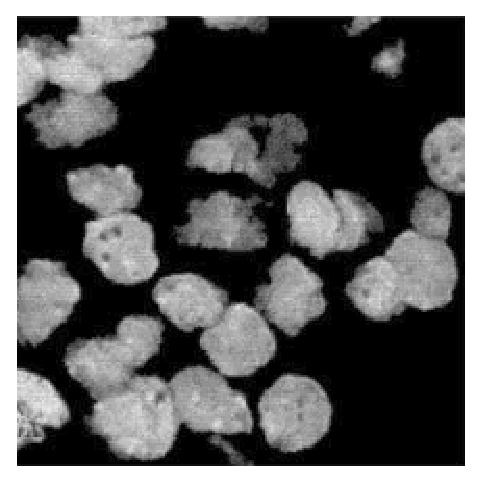
\includegraphics[width=0.33\textwidth]{pictures/watershedPrefiltb}\label{fig:watershedPrefiltb}}\\
\subfloat[][]{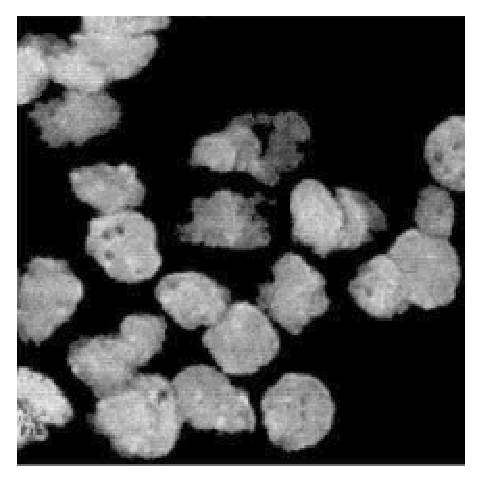
\includegraphics[width=0.33\textwidth]{pictures/watershedPrefiltc}\label{fig:watershedPrefiltc}}\hspace{5pt}
\subfloat[][]{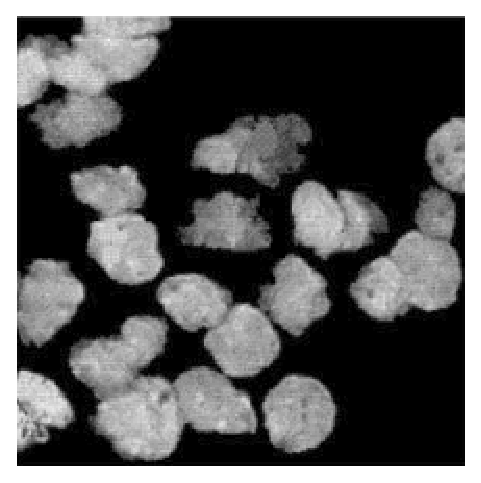
\includegraphics[width=0.33\textwidth]{pictures/watershedPrefiltd}\label{fig:watershedPrefiltd}}
\caption{Illustrations from \cite{umesh2001efficient}: Result of image enhancement steps shown over a single image slice:\\
\subref{fig:watershedPrefilta}: original image slice;
\subref{fig:watershedPrefiltb}: result of window slicing;
\subref{fig:watershedPrefiltc}: result of size-filtering;
\subref{fig:watershedPrefiltd}: result of morphological opening and closing of a 3D image.}
  \label{fig:watershedIllustration}
\end{figure}

\clearpage

\subsection*{Histological cell nuclei detection}
\label{sect:farsight}
Yousef Al-Kofahi {\etal}~\cite{al2009improved}, presents a new method for nuclei detection.
  \begin{description}
  \item[Data] are 2D histological images (see figure~\ref{fig:farsightInitial}).
  \item[Method] is described figure~\ref{fig:farsightFlowchart}.
  A first step consists in finding the foreground of the image with a graph cut based binarization (illustrated figure~\ref{farsightBinary}).
  A distance map is then computed on this binary image, and is used to constrain the scales of a multiscale Laplacian of Gaussian (see~\ref{sect:MLOG}).
  The original image is processed by the scale-constrained multi-scale Laplacien of Gaussian.
  A local maxima detection is performed on the resulting scalar field (as shown figure~\ref{fig:farsightMLOG}).
  Those local maximas correspond to the position of the cell.
  A watershed algorithm is then initiated from these points, and finally refined by manual editing and "alpha-refinement".
  \item[Evaluation] is done on 25 images containing an average of 298 cells per image. The results present the number of over and under segmented cell nuclei and separates encroachment errors.
  \item[Results] the algorithm provides acceptable results : 13.7\% of error.
  \item[Comments]: this article is well presented with a description of all the steps of the processing pipeline.
  The evaluation is done on enough images, and the results are detailed.
  The algorithm was implemented in the Farsight toolkit (FTK, \url{http://www.farsight-toolkit.org/}), but we were unable to make it run on 3D data.
\end{description}
\begin{figure}[h]
\begin{center}
\leavevmode
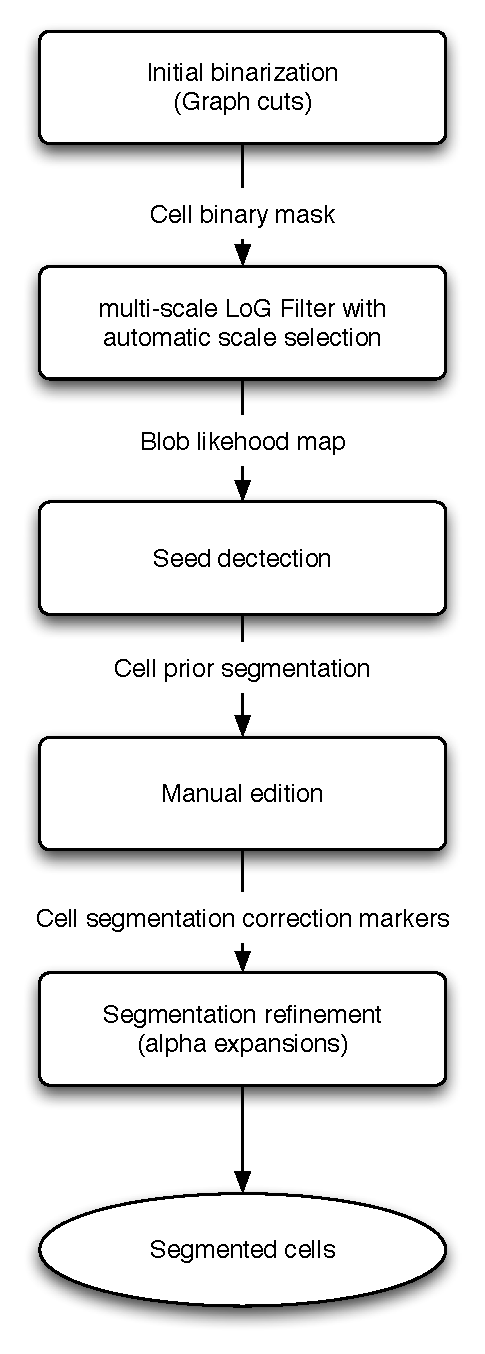
\includegraphics[height=0.87\textheight]{pictures/farsightFlowchart}
\end{center}
\caption{Flowchart of the algorithm proposed in~\cite{al2009improved}}
\label{fig:farsightFlowchart}
\end{figure}
\begin{figure}[h]
  \centering
  \captionsetup[subfloat]{labelformat=empty}
\subfloat[][]{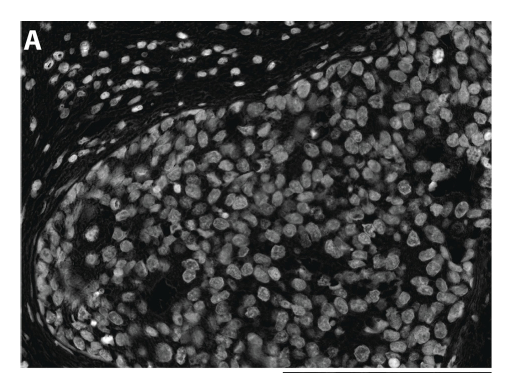
\includegraphics[width=0.49\textwidth]{pictures/farsightInitial}\label{fig:farsightInitial}}%
\subfloat[][]{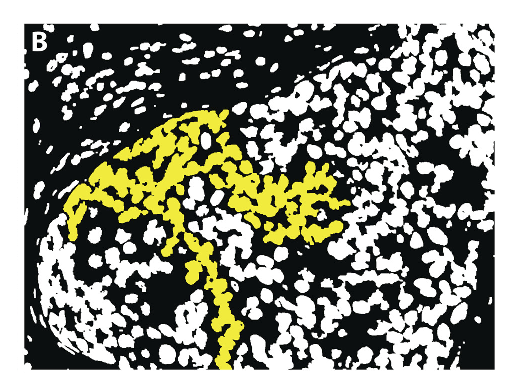
\includegraphics[width=0.49\textwidth]{pictures/farsightBinary}\label{fig:farsightBinary}} \\
\subfloat[][]{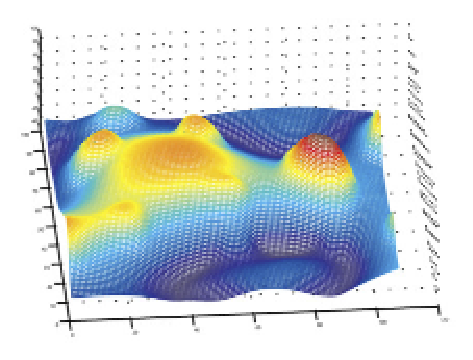
\includegraphics[width=0.33\textwidth]{pictures/farsightMLOGc}\label{fig:farsightMLOGc}}\hspace{5pt}
\subfloat[][]{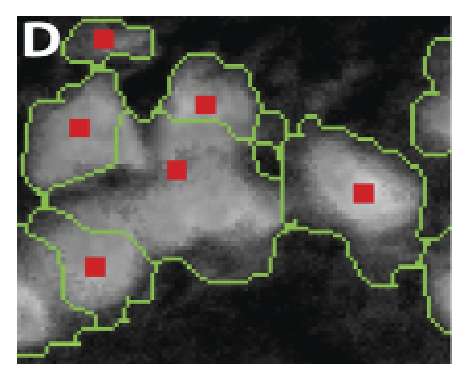
\includegraphics[width=0.33\textwidth]{pictures/farsightMLOGd}\label{fig:farsightMLOGd}}\\
\subfloat[][]{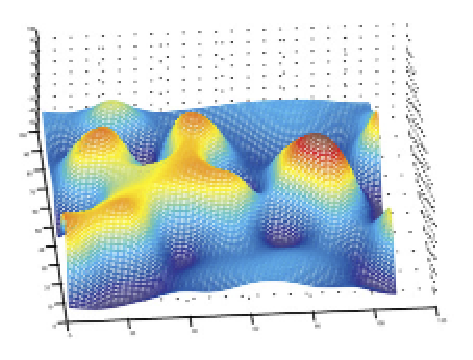
\includegraphics[width=0.33\textwidth]{pictures/farsightMLOGe}\label{fig:farsightMLOGe}}\hspace{5pt}
\subfloat[][]{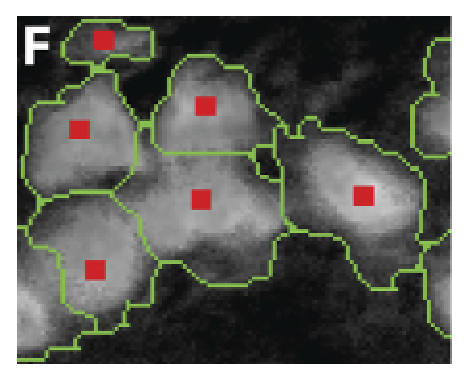
\includegraphics[width=0.33\textwidth]{pictures/farsightMLOGf}\label{fig:farsightMLOGf}}
%
\caption{%
illustrations from \cite{al2009improved}:\\
\subref{fig:farsightInitial}: Foreground extraction results. Pixels marked yellow represent a large connected component;
\subref{fig:farsightBinary}: Nuclear channel from spectral unmixing;
\subref{fig:farsightMLOGc}: Surface plot of the multiscale LoG filtering results for a small region;
\subref{fig:farsightMLOGd}:  Initial segmentation based on the LoG;
\subref{fig:farsightMLOGe}: Surface plot of the distance-map-constrained multiscale LoG;
\subref{fig:farsightMLOGf}:  Improved initial segmentation resulting from the distance-constrained LoG.
}
  \label{fig:farsightIllustration}
\end{figure}
\clearpage

%
%%\subsection*{Loukas two observers}
%%
%% C.G. Loukas {\etal}~\cite{loukas2003image}, published an article about automatic counting of cancer cell nuclei in tissue sections.
%%As their data is very different from ours, the main interest of this article is the evaluation method based on based on two observers.
%%  They count the number of cells in ten images and the average number of cell counting error of the algorithm in percent the average number of cell present in the images is given (150). No information is provided on evaluating the cell nuclei position, or on the type of error : over detection or under detection ? The data are histological sections (2D).
%
%\begin{description}
%  \item[Data] are histological sections from cell cancers.
%  \item[Method] is based on a modified Laplacian of Gaussian filtering with maxima detector. The data being extremely different from ours, the method is not further described in this report.
%
%  \item[Evaluation] is performed on 10 confocal datasets. The mean amount of nuclei in the datasets is 310. The number of over segmented and under segmented nuclei is presented. The automatic segmentation result is compared with the segmentation of two experts.
%  \item[Results] the algorithm provides good results in the paper: 
%  4.93\% of over-segmented nuclei,
%  and 5.03\% of under-segmented nuclei.
%  \item[Comments]: this article is well presented and evaluated,
%  equations and references are given for algorithm reproduction.
%  A windows executable of the algorithm is also provided. The code source is not released though. 
%  The article misses the part desrcibing the region cropping for getting the regions where the adaptive
%   threshold should be computed. 
%   Looking at the illustration, it seems like these regions are either determined 
%   according to attraction basins of each sink, or with a constrained Voronoi diagram.
%\end{description}
%
%
%

\subsection*{Existing method in the Megason Lab}
\label{sect:megasonExisting}
The existing method in the Megason Lab, for nuclei detection and segmentation, is also based on a detection of nuclei, and then, a segmentation, using watershed.
  \begin{description}
  \item[Data] are the challenging 3D confocal/2-photons images presented in the Data analysis part. 
  \item[Method] is described figure~\ref{fig:kishoreFlowchart},
  A pre processing stage consists in denoising the raw image, with an anisotropic diffusion filter.
  Then, the algorithm consists in a combination of methods : 
  hough transform, image masking and distance map, and the redial voting technique described in \cite{chang2007segmentation}, applied to the denoised image.
  Once the three filters processed the nuclei image, their output scalar fields are summed.
  A local maxima extraction is performed on this resulting field.
  This extraction filters the close local maximas, to reduce the noise impact, by selecting the highest local maxima, and ignoring the other local maximas in a certain radius.
  those maximas are then used for initializing a watershed algorithm.
  \item[Evaluation] has been visually carried out by Kishore, for the initialization points of the watershed.
  For the result of the watershed, the evaluation was performed on an expert-segmented dataset of 180 cell nuclei.
  \item[Results] are still to be evaluated.
  \item[Comments]: there is an existing method in the Megason lab, but it has not yet been evaluated nor published. Improving this method consists in, first going through the algorithms' code, then create a visualization and evaluation framework, and finally compare it with other methods.
\end{description}
\begin{figure}[h]
\begin{center}
\leavevmode
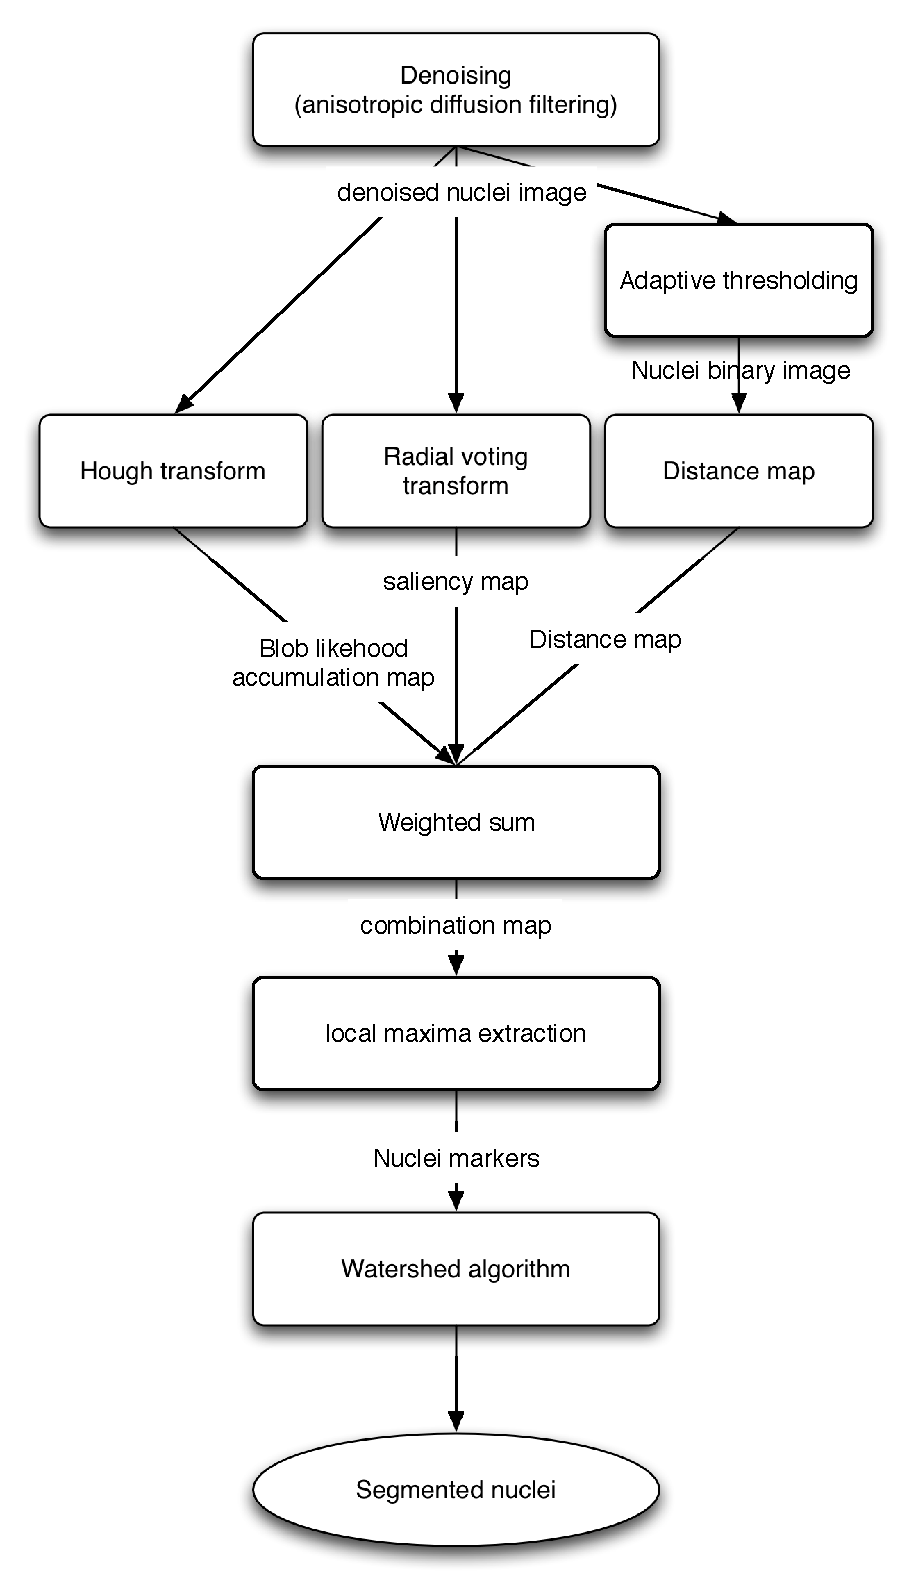
\includegraphics[height=0.87\textheight]{pictures/kishoreFlowchart}
\end{center}
\caption{Flowchart of the algorithm used in the Megason Lab}
\label{fig:kishoreFlowchart}
\end{figure}
\clearpage


\subsection*{Conclusion}

We can conclude that there are some existing algorithms for detecting and segmenting cell nuclei,
but very few were designed for 3D confocal data.
Most of the time, they perform well on 2D datasets, but are tricked by the low resolution of the third dimension.
The evaluation is most of times based on the final segmentation, and interesting informations are number of over/under-segmented cell nuclei.



